\documentclass{beamer}
\usepackage{../common_slides}
\usepackage{tikz}
\usepackage{tikz-qtree}
\usepackage{pdfpages}

\usetikzlibrary{matrix}
% \usepackage{enumitem}

\title{Sequence Models 3}
\date{}
\author{CS 287}

\def\Lattice{
    \matrix (network)
    [matrix of nodes,
    nodes in empty cells,
    ampersand replacement=\&,
    column sep={1cm},
    row sep={0.1cm},
    nodes={outer sep=0pt,circle,minimum size=0.5cm, minimum width=1.3cm,draw, rectangle} ]
    {
     O \& O \& O \& O \& O\\
     I-PER \& I-PER \& I-PER \& I-PER \& I-PER \\ 
     I-ORG \& I-ORG \& I-ORG \& I-ORG \& I-ORG \\ 
     I-LOC \& I-LOC \& I-LOC \& I-LOC \& I-LOC \\ 
     |[draw=none]| \\
     |[draw=none]| Mayor \& |[draw=none]| DeBlasio \& |[draw=none]| from \& |[draw=none]| New  \& |[draw=none]| York  \\  
};
}



\def\LatticeB{
    \matrix (network)
    [matrix of nodes,
    nodes in empty cells,
    ampersand replacement=\&,
    column sep={1cm},
    row sep={0.1cm},
    nodes={outer sep=0pt,circle,minimum size=0.5cm, minimum width=1.3cm,draw, rectangle} ]
    {
     O \& O \& O \& O \& O\\
     I \& I \& I \& I \& I \\ 
     |[draw=none]| \\
     |[draw=none]| Mayor \& |[draw=none]| DeBlasio \& |[draw=none]| from \& |[draw=none]| New  \& |[draw=none]| York  \\  
};
}

\begin{document}
\begin{frame}
  \titlepage
\end{frame}

\begin{frame}{Review: Markov Models}
  \begin{itemize}
  \item In general, intractable to solve sequence prediction,
 
  \[ \argmax_{c_{1:n}} f(\boldx, c_{1:n}) \] 

  \item Today, focus on (first-order) Markov models,

  \[ f(\boldx, c_{1:n})  = \sum_{i=1}^n \log \hat{y}(c_{i-1})_{c_i}\] 

  \item Can extend these ideas to higher-order models.

  \[ f(\boldx, c_{1:n})  = \sum_{i=1}^n \log \hat{y}(c_{i-2}, c_{i-1})_{c_i}\] 
  \end{itemize}  
  
\end{frame}


\begin{frame}{Review: Greedy Search}
    \[ f(\boldx, c_{1:n})  = \sum_{i=1}^n \log \hat{y}(c_{i-1})_{c_i} \] 

    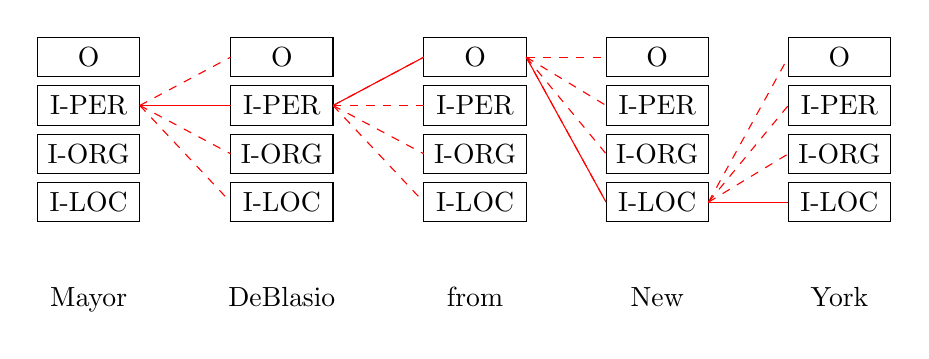
\begin{tikzpicture}
    \Lattice
    \draw<2->[red] (network-2-1.east) --  (network-2-2.west);
    \draw<3->[red] (network-2-2.east) -- (network-1-3.west); 
    \draw<4->[red] (network-1-3.east) -- (network-4-4.west);
    \draw<5->[red] (network-4-4.east) -- (network-4-5.west);

    \foreach \j in {1,...,4} {
    \draw<1>[red,dashed] (network-2-1.east) -- (network-\j-2.west);
    \draw<2>[red,dashed] (network-2-2.east) -- (network-\j-3.west);
    \draw<3>[red,dashed] (network-1-3.east) -- (network-\j-4.west);
    \draw<4>[red,dashed] (network-4-4.east) -- (network-\j-5.west);
    } 

    \end{tikzpicture}
\end{frame}



\begin{frame}{Review: Dynamic Programming over a Lattice}
  \begin{itemize}
  \item Several different varieties: Viterbi, forward, backward

  \item Recursive Definition:
    \begin{itemize}
    \item Base Case: Start with the score for sequence of length 1.  \air
    \item Inductive Case: Compute all sequences of length $i$ from $i-1$ 
    \end{itemize}
  \end{itemize}

  \begin{center}   
  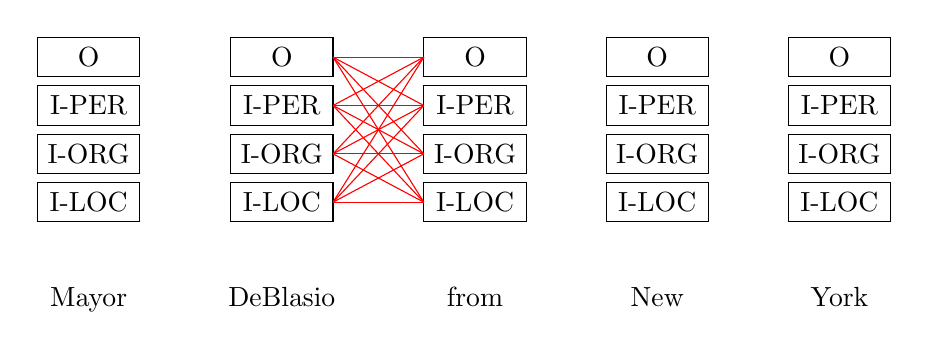
\begin{tikzpicture}
    \Lattice
    \foreach \i in {1,...,4} {
    \foreach \j in {1,...,4} {
    \draw[red] (network-\i-2.east) -- (network-\j-3.west);
    } }
  \end{tikzpicture}
  \end{center}  
\end{frame}


\begin{frame}{Review: Viterbi Algorithm}
  \begin{algorithmic}
    \Procedure{Viterbi}{}
    \State{$\pi \in \reals^{ (n+1) \times \mcC}$ initialized to $-\infty$ }
    \State{$\pi[0, \langle s \rangle] = 0$}
    \For{$i = 1$ to $n$ }
    \For{$c_{i} \in \mcC$}
    \State{$\pi[i, c_i] = \max_{c_{i-1}} 
     \pi[i-1, c_{i-1}] + \log \hat{y}(c_{i-1})_{c_i}        
       $}
    \EndFor{}
    \EndFor{}
    \State{\Return{$\max_{c_n\in\mcC} \pi[n, c_n]$}}
    \EndProcedure{}
  \end{algorithmic}
  \begin{itemize}
  \item Time Complexity?
  \item Space Complexity?
  \end{itemize}
\end{frame}

\begin{frame}{Quiz: Reverse it}
  Each of the algorithms goes left-to-right (forward) when producing 
  a sequence. Sometimes you can derive right-to-left versions 
  of these algorithms. Consider right-to-left cases of the 
  following. Which are possible to run, how does the algorithm change, and 
  do you get the same solutions?

  \begin{enumerate}
  \item Right-to-left greedy search on a Markov model.
  \item Right-to-left Viterbi search on a Markov model.
  \item Right-to-left greedy search on an RNN model
  \end{enumerate}

\end{frame}

\begin{frame}{Answer: R-to-L Greedy Search}
  \begin{itemize}
  \item In general, may not work. 
    
  \item May require computing and renormalizing one step in the past ($O(|\mcC|^2)$)

  \item Likely gives a different solution than forward greedy. 
  \end{itemize}

  \begin{center}
    \begin{algorithmic}
      \Procedure{GreedySearch}{} \State{$s = 0$} \Comment{Running score}
      \State{$c_{n+1} = \langle /s \rangle$} \Comment{Final Symbol}
      \For{$i = n$ to $1$ }
      \State{$c_i \gets\displaystyle \argmax_{c'_i} \alert{\hat{y}(c'_{i})_{c_{i+1}}}$}
      \State{$s \gets s + \log \hat{y}(c_{i})_{c_{i+1}}$}
      \EndFor{}
      \State{\Return{$c, s$}}
      \EndProcedure{}
    \end{algorithmic}
  \end{center}
\end{frame}

\begin{frame}{Answer: R-to-L Greedy Search (worst-case)}
    \[ f(\boldx, c_{1:n})  = \sum_{i=1}^n \log \hat{y}(c_{i-1})_{c_i} \] 

    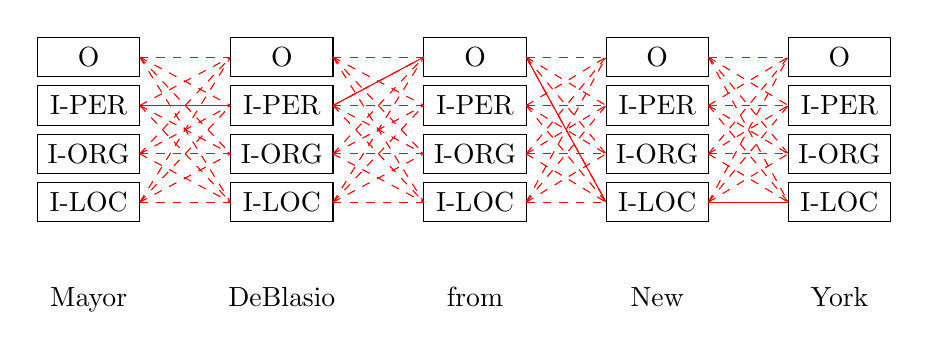
\begin{tikzpicture}
    \Lattice
    \draw<5->[red] (network-2-1.east) --  (network-2-2.west);
    \draw<4->[red] (network-2-2.east) -- (network-1-3.west); 
    \draw<3->[red] (network-1-3.east) -- (network-4-4.west);
    \draw<2->[red] (network-4-4.east) -- (network-4-5.west);

    \foreach \j in {1,...,4} {
      \foreach \i in {1,...,4} {
        \draw<4>[red,dashed] (network-\j-1.east) -- (network-\i-2.west);
      
        \draw<3>[red,dashed] (network-\j-2.east) -- (network-\i-3.west);
        \draw<2>[red,dashed] (network-\j-3.east) -- (network-\i-4.west);
        \draw<1>[red,dashed] (network-\j-4.east) -- (network-\i-5.west);
      }
    } 
    \end{tikzpicture}
\end{frame}

\begin{frame}{Answer: Backward Viterbi}
  \begin{itemize}
  \item Same speed, same results.
  \item Similar inductive rule applies.
  \item Construct sequences starting at the end. 
  \end{itemize}

  \begin{algorithmic}
    \Procedure{BackwardViterbi}{}
    \State{$\pi \in \reals^{ (n+1) \times \mcC}$ initialized to $-\infty$ }
    \State{$\pi[n+1, \langle /s \rangle] = 0$}
    \For{$i = n$ to $1$ }
    \For{$c_{i} \in \mcC$}
    \State{$\pi[i, c_i] = \max_{c'_{i+1}} 
     \pi[i+1, c'_{i+1}] + \log \hat{y}(c_{i})_{c'_{i+1}}        
       $}
    \EndFor{}
    \EndFor{}
    \State{\Return{$\max_{c_1\in\mcC} \pi[1, c_1]$}}
    \EndProcedure{}
  \end{algorithmic}
\end{frame}

\begin{frame}{Backward Viterbi}
  \begin{center}
   
  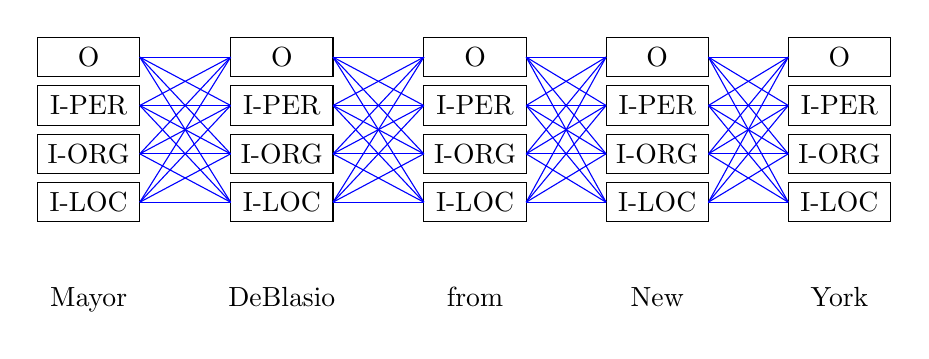
\begin{tikzpicture}
    \Lattice
    \foreach \i in {1,...,4} {
    \foreach \j in {1,...,4} {
    % \draw<1->[red] (network-\i-1.east) -- (network-\j-2.west);
    % \draw<2->[red] (network-\i-2.east) -- (network-\j-3.west);
    % \draw<3->[red] (network-\i-3.east) -- (network-\j-4.west);
    % \draw<4->[red] (network-\i-4.east) -- (network-\j-5.west);
    \draw<5->[blue] (network-\i-1.east) -- (network-\j-2.west);
    \draw<4->[blue] (network-\i-2.east) -- (network-\j-3.west);
    \draw<3->[blue] (network-\i-3.east) -- (network-\j-4.west);
    \draw<2->[blue] (network-\i-4.east) -- (network-\j-5.west);

    } }
  \end{tikzpicture}
  \end{center}  
\end{frame}


\begin{frame}{Answer: Right-to-Left Greedy RNN }
  \begin{itemize}
  \item Does not work. 
    \air
  \item Have suffix $c_n \ldots c_i$ but RNN is prefix-function  $\hat{\boldy}(c_1, \ldots c_i)$.
    \air 
  \item Backward greedy would require enumerating all prefixes. 
  \end{itemize}
\end{frame}

\begin{frame}{Alternative Solution: Backward RNN}
  \begin{itemize}
  \item Can train RNN in the reverse direction.
    \air
  \item RNN suffix transducer trained on $\hat{\boldy}(c_n, \ldots c_i)$.
    \air 
  \item However note this is a \structure{different} model. 
    \air
  \item Even if you had exact search, this may yield a different output.
  \end{itemize}
\end{frame}


\begin{frame}{Today's Lecture}
  \begin{itemize}
  \item More Dynamic Programming
    \begin{itemize}     
      \air 

    \item Max-Marginals
      \air

    \item Forward-Backward
      \air

    \item Probabilistic Marginals
      \air 
    \item Pruning 
    \end{itemize}
    \air 

  \item Next Lecture: Conditional Random Fields
  \end{itemize}
\end{frame}


% \begin{frame}{}
%   Sequence scoring function: 
%   \[ f(\boldx, c_{1, n}) \] 

%   \begin{itemize}
%   \item Takes an input $\boldx$ and a sequence $c_{1:n}$ gives a score.
%     \air 
%   \item Last lecture \[ \argmax_{c_{1:n}} f(\boldx, c_{1:n}) \]
%     \air
%   \item Other queries of interest. 
   
%   \end{itemize}
% \end{frame}

\begin{frame}{Question 1: Tag Fill-In}
  Assume we are given $c_{1:i-1}$ and $c_{i+1:n}$,
  \air 

  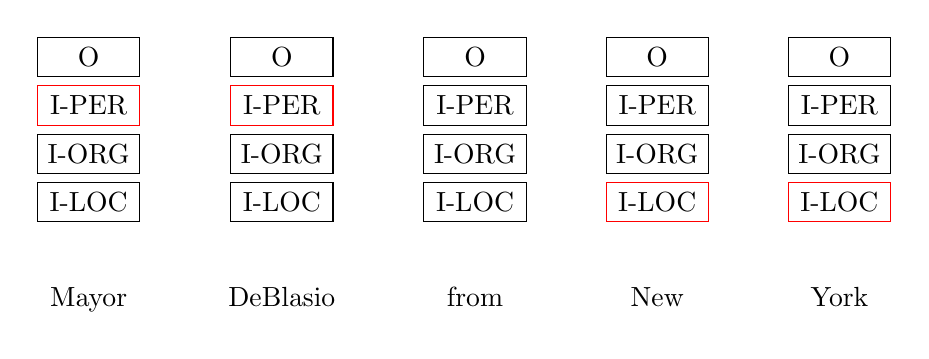
\begin{tikzpicture}
    \Lattice
    \draw[red] (network-2-1.north west) rectangle  (network-2-1.south east);
    \draw[red] (network-2-2.north west) rectangle  (network-2-2.south east);
    \draw[red] (network-4-4.north west) rectangle  (network-4-4.south east);
    \draw[red] (network-4-5.north west) rectangle  (network-4-5.south east);
  \end{tikzpicture}
  \air
  \pause
  
  What is the best completion, i.e. 
  \[ \argmax_{c'_i} f(\boldx, c_{1:i-1}:c'_i:c_{i+1:n}) \] 
\end{frame}

\begin{frame}{Answer}
  \begin{itemize}
  \item Markov model. Score involving $c_i$ are local ($c_{i-1}$ and $c_{i+1}$).
    \air 

  \item   Can solve by looking one-step forward and backward

    \[ \argmax_{c'_i} f(\boldx, c_{1:n})  = \argmax_{c'_i} \log \hat{y}(c_{i-1})_{c'_i} + \log \hat{y}(c'_{i})_{c_{i+1}} \] 
    \air 

  \item Can be solved in $O(|\mcC|)$ or $O(|\mcC|^2)$ depending on model.
  \end{itemize}
\end{frame}


\begin{frame}{Exercise 2: Sequence fill-in}
  Assume we \textbf{are not} given $c_{1:i-1}$ and $c_{i+1:n}$,
  \air 

  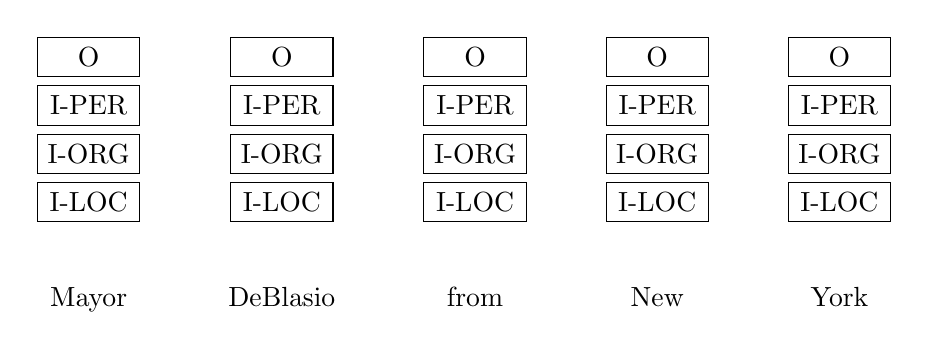
\begin{tikzpicture}
    \Lattice
    % \draw[red] (network-2-1.north west) rectangle  (network-2-1.south east);
    % \draw[red] (network-2-2.north west) rectangle  (network-2-2.south east);
    % \draw[red] (network-4-4.north west) rectangle  (network-4-4.south east);
    % \draw[red] (network-4-5.north west) rectangle  (network-4-5.south east);
  \end{tikzpicture}

  What is the score of the max sequence through each tag, i.e. 
  \[ M(i, c'_i) = \max_{c_{1:i-1},c_{i+1:n}} f(\boldx, c_{1:i-1}:c'_i:c_{i+1:n}) \] 
\end{frame}

\begin{frame}{Answer}
  \begin{itemize}
  \item Markov property. Two prefix and suffix score can are independent.
    \air 

  \item   
    \begin{eqnarray*}
      M(i, c'_i) &=& \max_{c_{1:i-1}:c_{i+1:n}} f(\boldx, c_{1:i-1}:c'_i:c_{i+1:n})  \\
       &=& \max_{c_{1:i-1}} \log \hat{y}(c'_{i-1})_{c'_{i}} + \sum_{j=1}^i \log  \hat{y}(c_{j-1})_{c_{j}}   \\
       &+& \max_{c_{i+1:n}} \log \hat{y}(c'_{i})_{c_{i+1}} +  \sum_{j=i+1}^n \log \hat{y}(c_{j})_{c_{j+1}}  
    \end{eqnarray*}

  \end{itemize}
\end{frame}

\begin{frame}{Viterbi Forward-Backward}
    \begin{eqnarray*}
       &&\max_{c_{1:i-1}} \log \hat{y}(c'_{i-1})_{c'_{i}} + \sum_{j=1}^i \log  \hat{y}(c_{j-1})_{c_{j}}   \\
       &+& \max_{c_{i+1:n}} \log \hat{y}(c'_{i})_{c_{i+1}} +  \sum_{j=i+1}^n \log \hat{y}(c_{j})_{c_{j+1}}  
    \end{eqnarray*}

   \begin{itemize}
  \item  Forward Viterbi scores (max prefix)
    \[  \pi^{\alpha}[i, c'_i]  = \max_{c_{1:i-1}} \log \hat{y}(c'_{i-1})_{c'_{i}} + \sum_{j=1}^i \log  \hat{y}(c_{j-1})_{c_{j}}   \]
    
    
    \air
  \item  Backward Viterbi scores (max suffix)
     \[ \pi^{\beta}[i, c'_i] = \max_{c_{i+1:n}} \log \hat{y}(c'_{i})_{c_{i+1}} +  \sum_{j=i+1}^n \log \hat{y}(c_{j})_{c_{j+1}} \]

   \end{itemize}
\end{frame}

\begin{frame}
  \begin{center}

  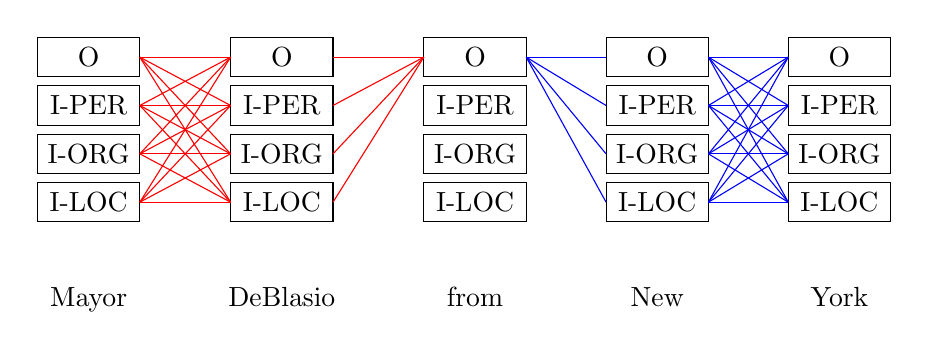
\begin{tikzpicture}
    \Lattice

    \draw[blue] (network-1-3.east) -- (network-1-4.west);
    \draw[blue] (network-1-3.east) -- (network-2-4.west); 
    \draw[blue] (network-1-3.east) -- (network-3-4.west);
    \draw[blue] (network-1-3.east) -- (network-4-4.west);

    \draw[red] (network-1-3.west) -- (network-1-2.east);
    \draw[red] (network-1-3.west) -- (network-2-2.east); 
    \draw[red] (network-1-3.west) -- (network-3-2.east);
    \draw[red] (network-1-3.west) -- (network-4-2.east);

    \foreach \i in {1,...,4} {
    \foreach \j in {1,...,4} {
    \draw[red] (network-\i-1.east) -- (network-\j-2.west);
    % \draw[red] (network-\i-2.east) -- (network-\j-3.west);
    % \draw[red] (network-\i-3.east) -- (network-\j-4.west);
    \draw[blue] (network-\i-4.east) -- (network-\j-5.west);
    } }

  \end{tikzpicture}
  \end{center}  
\end{frame}


\begin{frame}{Computing All Max-Marginals}
  \[ \argmax_{c_i} \max_{c_{1:i-1}:c_{i+1:n}} f(\boldx, c_{1:n}) \] 
  \begin{itemize}
  \item Compute $\pi^{\alpha}$ using Viterbi forward
    \air 

  \item Compute $\pi^{\beta}$ using Viterbi backward 
    \air

  \item Compute the argmax
    \[ M(i, c'_i) = \pi^{\alpha}[i, c'_i] + \pi^{\beta}[i, c'_i] \] 
  \end{itemize}
  
  \begin{itemize}
  \item Time complexity?
    \air 
  \item Space complexity?
  \end{itemize}
\end{frame}

\begin{frame}
  \begin{center}
   
  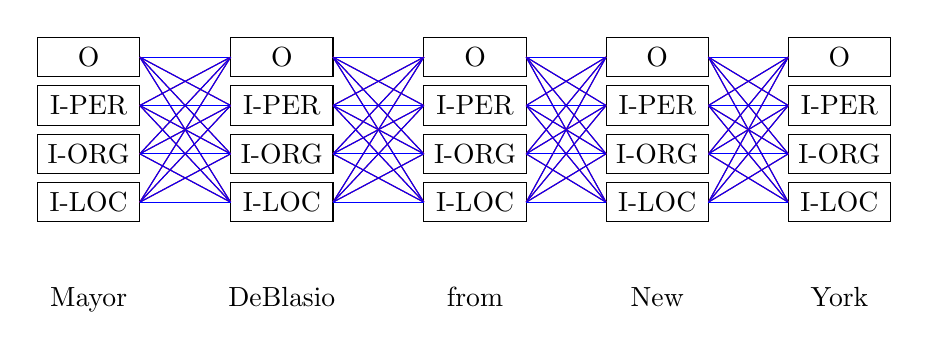
\begin{tikzpicture}
    \Lattice
    \foreach \i in {1,...,4} {
    \foreach \j in {1,...,4} {
    \draw<1->[red] (network-\i-1.east) -- (network-\j-2.west);
    \draw<2->[red] (network-\i-2.east) -- (network-\j-3.west);
    \draw<3->[red] (network-\i-3.east) -- (network-\j-4.west);
    \draw<4->[red] (network-\i-4.east) -- (network-\j-5.west);
    \draw<8->[blue] (network-\i-1.east) -- (network-\j-2.west);
    \draw<7->[blue] (network-\i-2.east) -- (network-\j-3.west);
    \draw<6->[blue] (network-\i-3.east) -- (network-\j-4.west);
    \draw<5->[blue] (network-\i-4.east) -- (network-\j-5.west);

    } }
  \end{tikzpicture}
  \end{center}  
\end{frame}



\begin{frame}{Max-Marginals with Backpointers}
  \begin{itemize}
  \item Can also include forward and backward backpointers
    \air 
  \item Get best sequence through any tag in $O(n|\mcC|^2)$. 
  \end{itemize}
\end{frame}

\begin{frame}{Max-Marginal Property}
  If $c^*_i$ is part of highest-scoring sequence then max-marginal at
  $M(i, c^*_i)$ is $\max_{c_{1:n}} f(\boldx, c_{1:n})$ and by definition is at
  least as large as any other max-marginal  $M(j, c_j)$ for all $j, c_j$.
\end{frame}


\begin{frame}{Pruning by Bounding (Sketch)}
  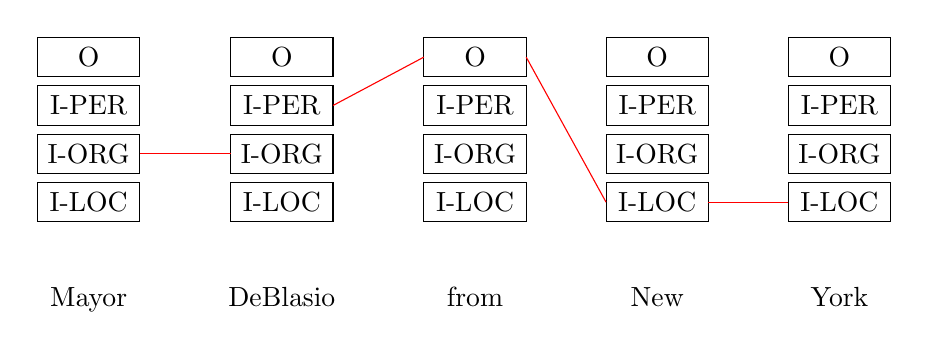
\begin{tikzpicture}
    \Lattice
    \draw[red] (network-3-1.east) --  (network-3-2.west);
    \draw[red] (network-2-2.east) -- (network-1-3.west); 
    \draw[red] (network-1-3.east) -- (network-4-4.west);
    \draw[red] (network-4-4.east) -- (network-4-5.west);

  \end{tikzpicture}
  \begin{itemize}
  \item First run greedy over full problem.
    \air 
  \item Score $s^{(greedy)}$ is less than optimal.  
  \end{itemize}
\end{frame}


\begin{frame}{Pruning by Bounding (Sketch)}
  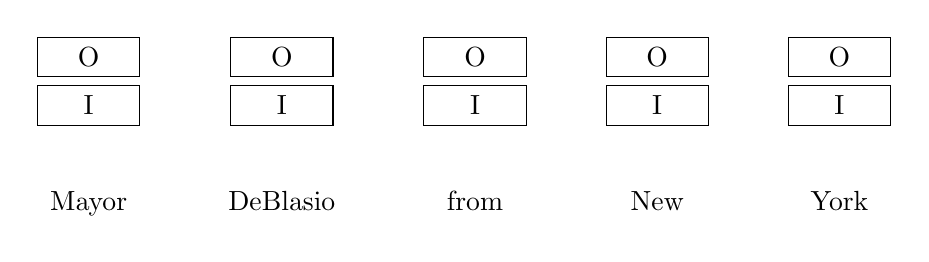
\begin{tikzpicture}
    \LatticeB
  \end{tikzpicture}
  \begin{itemize}
  \item Each edge is the \structure{max} of the edges in the full lattice.
    \air 

  \item Can compute max-marginals $M$ in much lkess time.
  \end{itemize}
\end{frame}

\begin{frame}{Pruning by Bounding (Sketch)}
  \begin{itemize}
  \item For all  $j, c_j$, if $M(j, c_j) < s^{greedy}$ can prune.
    \air
  \item Running Viterbi over pruned lattice is provably optimal.
    \air 
  \end{itemize}

  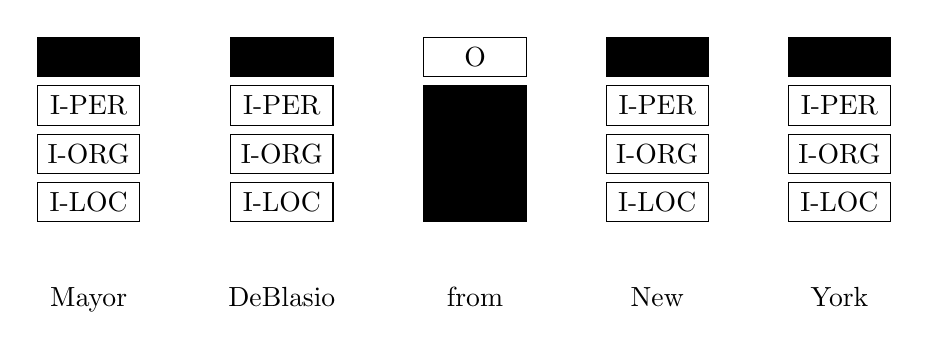
\begin{tikzpicture}
    \Lattice
    \draw[black, fill] (network-1-1.north west) rectangle  (network-1-1.south east);
    \draw[black, fill] (network-1-2.north west) rectangle  (network-1-2.south east);
    \draw[black, fill] (network-2-3.north west) rectangle  (network-4-3.south east);
    \draw[black, fill] (network-1-4.north west) rectangle  (network-1-4.south east);
    \draw[black, fill] (network-1-5.north west) rectangle  (network-1-5.south east);

    % \draw[black, fill] (network-2-1.north west) rectangle  (network-2-1.south east);
    % \draw[red] (network-2-2.north west) rectangle  (network-2-2.south east);
    % \draw[red] (network-4-4.north west) rectangle  (network-4-4.south east);
    % \draw[red] (network-4-5.north west) rectangle  (network-4-5.south east);

  \end{tikzpicture}
  
\end{frame}


% \begin{frame}{Using max-marginals}
%   \[ M(c_i) = \max_{c_{1:n}} f(\boldx, c_{1:n}) \] 
%   What if 
% \end{frame}


\section{Probabilistic Models}

\begin{frame}{Marginals}
  Let us return to the case of discriminative probabilistic models.
  \begin{itemize}
  \item Model of \[p(\boldy=\delta(c_{1:n}) | \boldx) \]
    \air 
  \item  

  \end{itemize}
\end{frame}

\begin{frame}{Exercise 3: Smoothing}
  Assume we are given $c_{1:i-1}$ and $c_{i+1:n}$, 
  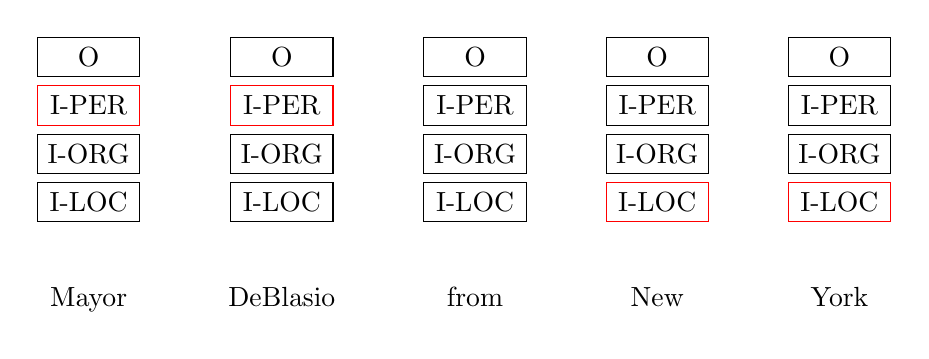
\begin{tikzpicture}
    \Lattice
        \draw[red] (network-2-1.north west) rectangle  (network-2-1.south east);
    \draw[red] (network-2-2.north west) rectangle  (network-2-2.south east);
    \draw[red] (network-4-4.north west) rectangle  (network-4-4.south east);
    \draw[red] (network-4-5.north west) rectangle  (network-4-5.south east);
  \end{tikzpicture}

  What is the probability of $\boldy_i$, i.e. 
  \[ p(\bold{y}_i = \delta(c_i) | \boldy_{1:i-1} = \delta(c_{1:i-1}), \boldy_{i+1:n} = \delta(c_{i+1:n}), \boldx ) \] 
\end{frame}

\begin{frame}{Answer}
  \begin{itemize}
  \item Same idea. Score involving $c_i$ are local ($i-1$ and $i+1$).
    \air 

  \item Can compute ``smoothing'' distribution from local information 
    \begin{eqnarray*}
      p(\bold{y}_i = \delta(c_i) | \boldy_{1:i-1}, \boldy_{i+1:n}, \boldx) &\propto& p(\bold{y}_i | \boldy_{i-1}) p(\boldy_{i+1} | \boldy_{i}) \\ 
      &=& \hat{y}(c_{i-1})_{c'_{i}} \hat{y}(c'_{i})_{c_{i+1}}
    \end{eqnarray*}

    \air 

  \end{itemize}
\end{frame}

\begin{frame}{Exercise 4}
  Assume we \textbf{are not} given $c_{1:i-1}$ and $c_{i+1:n}$.
  \air 

  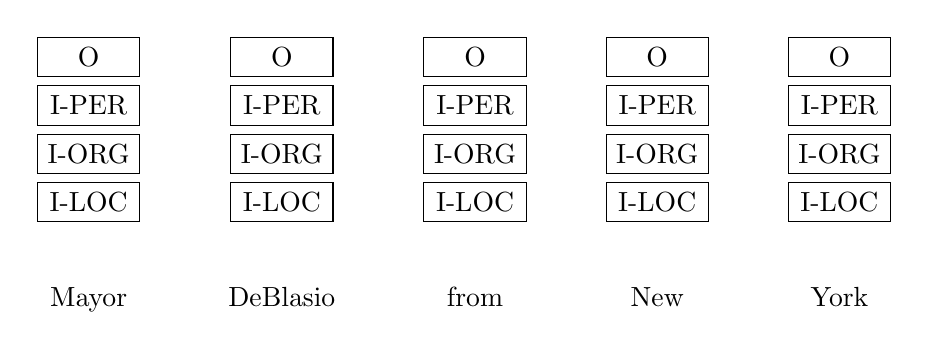
\begin{tikzpicture}
    \Lattice
    % \draw[red] (network-2-1.north west) rectangle  (network-2-1.south east);
    % \draw[red] (network-2-2.north west) rectangle  (network-2-2.south east);
    % \draw[red] (network-4-4.north west) rectangle  (network-4-4.south east);
    % \draw[red] (network-4-5.north west) rectangle  (network-4-5.south east);
  \end{tikzpicture}

  What is the best completed sequence, i.e. 
  \begin{eqnarray*}
    p(\boldy_i = \delta(c_i)| \boldx)
  \end{eqnarray*}
\end{frame}

\begin{frame}{Answer: Marginalization}
  \begin{itemize}
  \item Similar idea. Score involving $c_i$ are local ($i-1$ and $i+1$).
    \air 


    \begin{eqnarray*}
    p(\boldy_i = \delta(c'_i)| \boldx) &=& \sum_{c_{1:i-1}:c_{i+1:n}} p(\bold{y}_i = \delta(c'_i),  \boldy_{1:i-1,i+1:n}| \boldx ) \\ 
                                       &=& \sum_{c_{1:i-1}} p(\boldy_{1:i-1}|\boldx) p(\bold{y}_i = \delta(c'_i)|  \boldy_{i-1},  \boldx ) \\
                                       &\times&  \sum_{c_{i+1:n}} p(\bold{y}_{i+1}| \boldy_{i} = , \boldx) p(\bold{y}_{i+1:n}|\boldx) \\       \pause
                                       &= & \sum_{c_{1:i-1}} \hat{y}(c_{i-1})_{c'_{i}}  \prod_{j=1}^{i-1} \hat{y}(c_{j-1})_{c_{j}}  \\
                                       &\times& \sum_{c_{i+1:n}}  \hat{y}(c'_{i})_{c_{i+1}} \prod_{j=i+1}^n   \hat{y}(c_{j})_{c_{j+1}} \\      
      % \argmax_{c_i} \sum_{c_{1:i-1}:c_{i+1:n}} p(\bold{y}_i = \delta(c_i),  \boldy_{1:i-1} = \delta(c_{1:i-1}), \boldy_{i+1:n} = \delta(c_{i+1:n})| \boldx ) & = &  \argmax_{c_i} (\sum_{c_{1:i-1}} \sum_{j=1}^i \log \hat{\boldy}(c_{j-1})_{c_{j}} ))  \\
      % &+& (\sum_{c_{i:n}} \sum_{j=i+1}^n \log \hat{\boldy}(c_{j})_{c_{j+1}} ) \\      
    \end{eqnarray*}
    \air 
  \end{itemize}
\end{frame}

\begin{frame}{Forward and Backward}
  \begin{itemize}
  \item  Forward scores (sum over prefixes)
    \[ \alpha[i, c'_i] = \sum_{c_{1:i-1}} \hat{y}(c_{i-1})_{c'_{i}}  \prod_{j=1}^{i-1} \hat{y}(c_{j-1})_{c_{j}}  \]

    \air
  \item  Backward scores (sum over suffixes)
   \[ \beta[i, c'_i] = \sum_{c_{i+1:n}}  \hat{y}(c'_{i})_{c_{i+1}} \prod_{j=i+1}^n   \hat{y}(c_{j})_{c_{j+1}}  \]
  \end{itemize}
\end{frame}

\begin{frame}{Forward Algorithm}
  \begin{algorithmic}
    \Procedure{Forward}{}
    \State{$\alpha \in \reals^{\{0,\ldots, n\} \times \mcC}$  }
    \State{$\alpha[0, \langle s \rangle] = 1$}
    \For{$i = 1$ to $n$ }
    \For{$c_{i} \in \mcC$}
    \State{$\alpha[i, c_i] = \sum_{c_{i-1}} 
     \alpha[i-1, c_{i-1}] \times \hat{y}(c_{i-1})_{c_i}        
       $}
    \EndFor{}
    \EndFor{}
    \State{\Return{$\alpha$}}
    \EndProcedure{}
  \end{algorithmic}
\end{frame}


\begin{frame}{Backward Algorithm}
  \begin{algorithmic}
    \Procedure{Backward}{}
    \State{$\beta \in \reals^{\{1,\ldots, n+1\} \times \mcC}$}
    \State{$\beta[n+1, \langle s \rangle] = 1$}
    \For{$i = n$ to $1$ }
    \For{$c_{i} \in \mcC$}
    \State{$\beta[i, c_i] = \sum_{c_{i+1}} 
     \beta[i+1, c_{i+1}] \times \hat{y}(c_{i})_{c_{i+1}}        
       $}
    \EndFor{}
    \EndFor{}
    \State{\Return{$\beta$}}
    \EndProcedure{}
  \end{algorithmic}
\end{frame}


\begin{frame}{Exercise 5: Edge Marginals}
  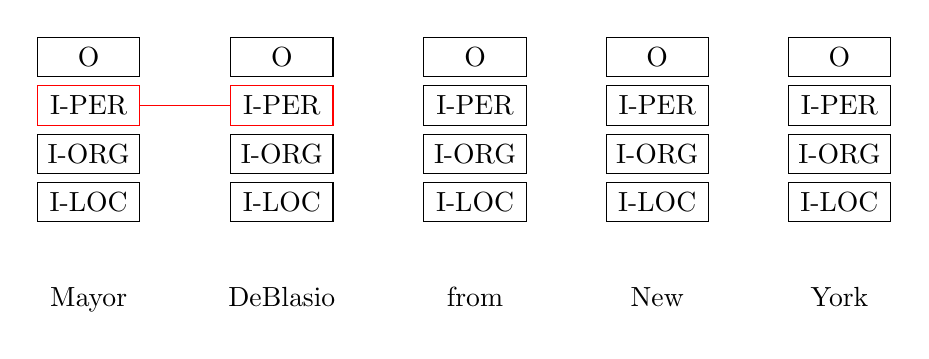
\begin{tikzpicture}
    \Lattice
    \draw[red] (network-2-1.north west) rectangle  (network-2-1.south east);
    \draw[red] (network-2-2.north west) rectangle  (network-2-2.south east);
    \draw[red] (network-2-1.east) --  (network-2-2.west);

    % \draw[red] (network-4-4.north west) rectangle  (network-4-4.south east);
    % \draw[red] (network-4-5.north west) rectangle  (network-4-5.south east);
  \end{tikzpicture}

  What is the probability of using an edge, i.e. 
 
  \[  p(\bold{y}_i = \delta(c'_i), \bold{y}_{i+1} = \delta(c'_{i+1}), | \boldx ) \] 

\end{frame}

\begin{frame}{Edge Marginals}
  \begin{eqnarray*}
    && \hat{y}(c'_{i})_{c'_{i+1}} \times \sum_{c_{1:i-1}} \hat{y}(c_{i-1})_{c'_{i}}  \prod_{j=1}^{i-1} \hat{y}(c_{j-1})_{c_{j}}  \\
     &\times& \sum_{c_{i+2:n}}  \hat{y}(c'_{i+1})_{c_{i+1}} \prod_{j=i+1}^n   \hat{y}(c_{j})_{c_{j+1}} \\          
  \end{eqnarray*}

  % \[ \argmax_{c_i, c_{i+1}} \max_{c_{1:i-1}:c_{i+2:n}} f(\boldx, c_{1:n}) \] 
  \begin{itemize}
  \item Compute $\alpha$ using Forward
    \air 

  \item Compute $\beta$ using Backward 
    \air

  \item Multiply in the edge 
    \[ \hat{y}(c'_{i})_{c'_{i+1}} \alpha[i, c'_i] \times \beta[i+1, c'_{i+1}] \] 
  \end{itemize}
  
  % \begin{itemize}
  % \item Time complexity?
  %   \air 
  % \item Space complexity?
  % \end{itemize}
\end{frame}


\begin{frame}{Edge Marginal}
  \begin{center}
   
  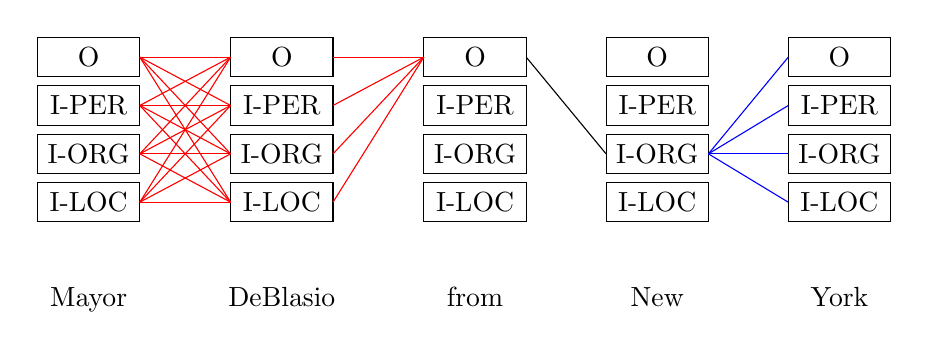
\begin{tikzpicture}
    \Lattice

    \draw[blue] (network-3-4.east) -- (network-1-5.west);
    \draw[blue] (network-3-4.east) -- (network-2-5.west); 
    \draw[blue] (network-3-4.east) -- (network-3-5.west);
    \draw[blue] (network-3-4.east) -- (network-4-5.west);
    \draw[black] (network-1-3.east) -- (network-3-4.west);

    \draw[red] (network-1-3.west) -- (network-1-2.east);
    \draw[red] (network-1-3.west) -- (network-2-2.east); 
    \draw[red] (network-1-3.west) -- (network-3-2.east);
    \draw[red] (network-1-3.west) -- (network-4-2.east);

    \foreach \i in {1,...,4} {
    \foreach \j in {1,...,4} {
    \draw[red] (network-\i-1.east) -- (network-\j-2.west);
    % \draw[red] (network-\i-2.east) -- (network-\j-3.west);
    % \draw[red] (network-\i-3.east) -- (network-\j-4.west);
    % \draw[blue] (network-\i-4.east) -- (network-\j-5.west);
    } }

  \end{tikzpicture}
  \end{center}  
\end{frame}



\begin{frame}{Marginals versus Max-Marginals}
  \begin{itemize}
  \item Max-Marginals: Most-likely sequence through decision
    \air 
  \item Marginals: Sum of sequences through decision.
  \end{itemize}
  \air 

  \begin{itemize}
  \item Possibly very different values.
    \air 

  \item Edge with highest marginal may not be in best sequence.
  \end{itemize}
\end{frame}



% \begin{frame}{Properties}
%   If $c^*_i$ is part of highest scoring sequence then max-marginal at
%   $c^i$ is $\max_{c_{1:n}} f(\boldx, c_{1:n})$ and by definition is at
%   least as large as any other max-marginal $c_j$.

%   Therefore, can read off best sequence from edge-marginals.

%   \textbf{however:} Not true for marginals.
% \end{frame}

% \begin{frame}{Node Marginal Decoding}
%   For all $c_i$ 
%   \[ \argmax_{c_i} p(y_i = \delta(c_i) | \boldx)   \] 

%   \begin{itemize}
%   \item Compute all node marginals.
%     \air 
%   \item Return most likely decision at each timestep.
%   \end{itemize}
% \end{frame}


\begin{frame}{Edge Marginal Decoding}
  \begin{itemize}
  \item   For all $i$ 
    \[  p(y_i = \delta(c_i), y_{i+1} = \delta(c_{i+1}) | \boldx)   \] 
  \item But this is a Markov model! 
    \air 

  \item Replace lattice with edge marginals 
    \[f(\boldx, c_{1:n}) = \sum_{i} \log p(y_i = \delta(c_i), y_{i+1} = \delta(c_{i+1}) | \boldx) \]

  \end{itemize}

  \begin{itemize}
  \item Posterior decoding.
    \[\argmax_{c_{1:n}} f(\boldx, c_{1:n}) \]
  \end{itemize}
\end{frame}






% \begin{frame}
  
% \end{frame}




% \begin{frame}
%   \begin{center}
   
%   \begin{tikzpicture}
%     \Lattice
%     \foreach \i in {1,...,4} {
%     \foreach \j in {1,...,4} {
%     \draw[red] (network-\i-1.east) -- (network-\j-2.west);
%     \draw[red] (network-\i-2.east) -- (network-\j-3.west);
%     \draw[red] (network-\i-3.east) -- (network-\j-4.west);
%     \draw[red] (network-\i-4.east) -- (network-\j-5.west);
%     } }

%     % \draw[red] (network-1-3.west) -- (network-1-2.east);
%     % \draw[red] (network-1-3.west) -- (network-2-2.east); 
%     % \draw[red] (network-1-3.west) -- (network-3-2.east);
%     % \draw[red] (network-1-3.west) -- (network-4-2.east);

%   \end{tikzpicture}
%   \end{center}  
  
% \end{frame}



% \begin{frame}
%   \begin{center}
   
%   \begin{tikzpicture}
%     \Lattice
%     \foreach \i in {1,...,4} {
%     \foreach \j in {1,...,4} {
%     \draw<8->[blue] (network-\i-1.east) -- (network-\j-2.west);
%     \draw<7->[blue] (network-\i-2.east) -- (network-\j-3.west);
%     \draw<6->[blue] (network-\i-3.east) -- (network-\j-4.west);
%     \draw<5->[blue] (network-\i-4.east) -- (network-\j-5.west);
%     } }
%   \end{tikzpicture}
%   \end{center}  
  
% \end{frame}


% \begin{frame}{Forward Algorithm}
%   \begin{algorithmic}
%     \Procedure{Forward}{}
%     \State{$\alpha \in \reals^{\{0,\ldots, n\} \times \mcC}$ initialized to $-\infty$ }
%     \State{$\alpha[0, \langle s \rangle] = 0$}
%     \For{$i = 1$ to $n$ }
%     \For{$c_{i} \in \mcC$}
%     \State{$\alpha[i, c_i] = \sum_{c_{i-1}} 
%      \alpha[i-1, c_{i-1}] * \hat{\boldy}(c_{i-1})_{c_i}        
%        $}
%     \EndFor{}
%     \EndFor{}
%     \State{\Return{$\sum_{c_n\in\mcC} \alpha[n, c_n]$}}
%     \EndProcedure{}
%   \end{algorithmic}
% \end{frame}


% \begin{frame}{Backward Algorithm}
%   \begin{algorithmic}
%     \Procedure{Backward}{}
%     \State{$\beta \in \reals^{\{1,\ldots, n+1\} \times \mcC}$ initialized to $-\infty$ }
%     \State{$\beta[n+1, \langle s \rangle] = 0$}
%     \For{$i = n$ to $1$ }
%     \For{$c_{i} \in \mcC$}
%     \State{$\beta[i, c_i] = \sum_{c_{i+1}} 
%      \beta[i+1, c_{i+1}] * \hat{\boldy}(c_{i})_{c_i+1}        
%        $}
%     \EndFor{}
%     \EndFor{}
%     \State{\Return{$\sum_{c_1\in\mcC} \beta[1, c_1]$}}
%     \EndProcedure{}
%   \end{algorithmic}
% \end{frame}





% \begin{frame}{Marginals}

%   \[M(c_i) =  \sum_{c_{1:n}} f(\boldx, c_{1:n}) \] 
  
%   % \[ \frac{\partial M}{\partial } \]

% \end{frame}


% \begin{frame}{Probabilistic }
%   \[ p(\boldy_i = c_i | \boldx) = \sum_{c_i} p( \boldy_i = \delta(c_i) | \boldx_{1:n})  \] 

%   For the case of MEMM gives you just this. 


%   For HMM
%   \begin{eqnarray*}
%      p(\boldy_i = c_i | \boldx) &=& \sum_{c_i} p( \boldy_i = \delta(c_i) | \boldx_{1:n})  \\
%      &= & p(\boldy_i = c_i | \boldx) = \sum_{c_i} p( \boldy_i = \delta(c_i), \boldx_{1:n}) / p(\boldx_{1:n})   
%   \end{eqnarray*}

%   How do you compute $p(\boldx_{1:n})$?
%   % \[M(c_i) =  \sum_{c_{1:n}} f(\boldx, c_{1:n}) \] 
  
%   % \[ \frac{\partial M}{\partial } \]

% \end{frame}

% \begin{frame}
%   \[ p(\boldx_{1:n}) = \sum_{c_i}  \] 
% \end{frame}


% \begin{frame}{Edge Marginals}

%   \[M(c_{i-1}, c_i) =  \sum_{c_{1:n}} f(\boldx, c_{1:n}) \] 
  
%   % \[ \frac{\partial M}{\partial } \]

% \end{frame}

% \begin{frame}{}
%   Is this the same forward-backward? 
% \end{frame}


% \begin{frame}{Viterbi}
  
  

% \end{frame}

% \section{Viterbi}
\end{document}